\documentclass{article}
\usepackage[utf8]{inputenc}
\usepackage{amsmath}
\usepackage{graphicx}
\usepackage{listings}
\begin{document}
\section{OpenMP}
In our serial adder, we quite straightforwadly sum our vector recursively, from the back of the vector and stores the sum in the beginning. Please don't watch to closely on the inline version.

The results from the serial implementation:
\begin{verbatim}
s = 1.6449340668
s - 2^3 	 0.1175120147
s - 2^4 	 0.0605875334
s - 2^5 	 0.0307668040
s - 2^6 	 0.0155035654
s - 2^7 	 0.0077820619
s - 2^8 	 0.0038986305
s - 2^9 	 0.0019512189
s - 2^10 	 0.0009760858
s - 2^11 	 0.0004881621
s - 2^12 	 0.0002441108
s - 2^13 	 0.0001220629
s - 2^14 	 0.0000610333
\end{verbatim}

\section{2.}
Our OpenMP parallelization is also quite straightforward. First we do some checks to catch some edge cases. Our sum is a basic paralell for loop with a reduction on sum.

\section{OpenMPI implementation }
Making an OpenMPI implementation we used the restrictions given in the assignment, which allow us to make a cleaner implementation. 

\begin{enumerate}

\item We do a number of iterations which is a power of two. 

\item We use a number of processes which is a power of two. 

\end{enumerate}

\begin{align}
2^{m}/2^{n} = 2^{m-n}
\end{align}

One effect of this is that we can partition the array, $2^{m}$ in the equation above, by dividing the size by the number of processes, $2^{n}$ above, to achieve the size of each partition, $2^{m-n}$. 
Since all these numbers can be represented as integers this gives no loss when doing integer division. 

We split the work into a few steps, populating the array, sending out the arrays to the workers, adding the elements of the arrays, sending back the answer, receiving the answer and summing the sums together. 

The primary thread is the only thread generating the array, it then sends all the other threads a piece of the array. 
Every other thread waits to receive its part. 
At this point every thread got one partition of the array, so they all find the sum of the contents in their partition. 
Every thread except the primary thread then proceeds to send the data back to the primary thread, which have been reveiving data from the threads and makes the final sum. 


\section{OpenMP and OpenMPI }
The differnce between the OpenMPI implementation and the combination is that the primary thread is using OpenMP to split the job into several senders and using the same technique for receiving. 
In addition the workers use OpenMP to paralellize their work. 


\begin{figure}
\caption{To achieve paralellization of reception we chose to use OpenMP's reduction in combination with {\tt MPI\_Receive}. This yields easy readable code which is paralellized. }
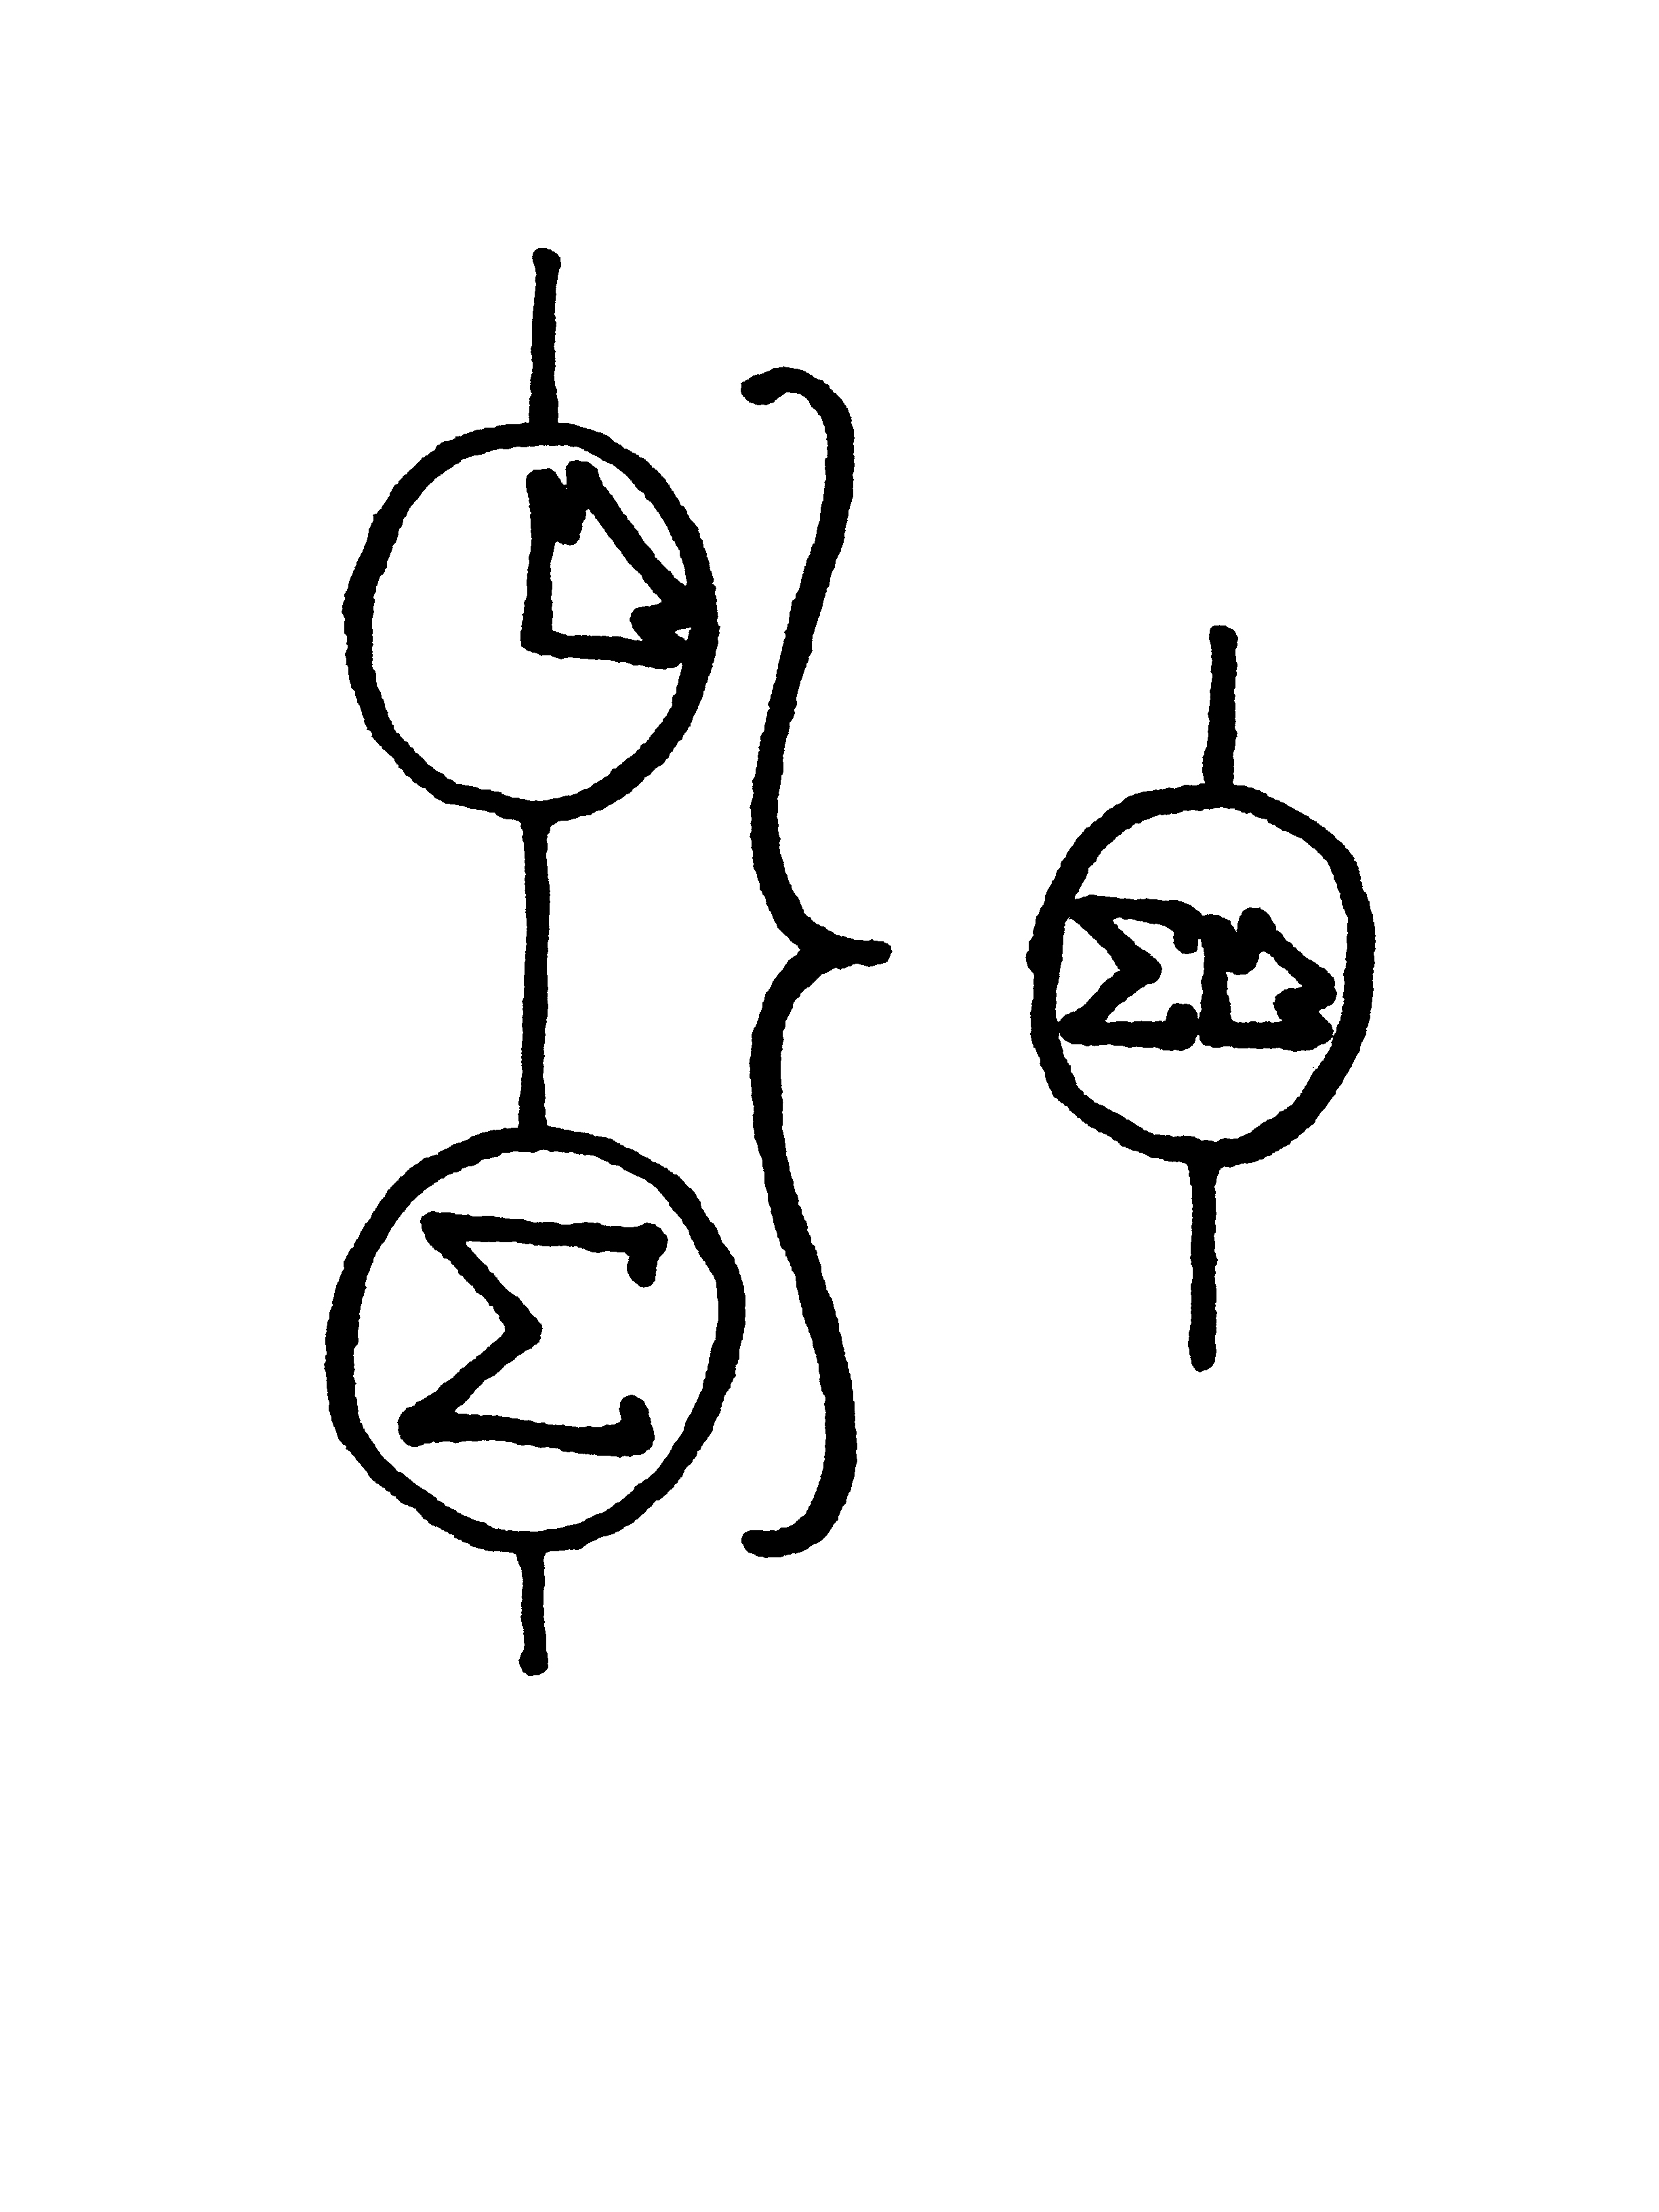
\includegraphics[width=\textwidth]{flyt2}
\end{figure}
\begin{figure}
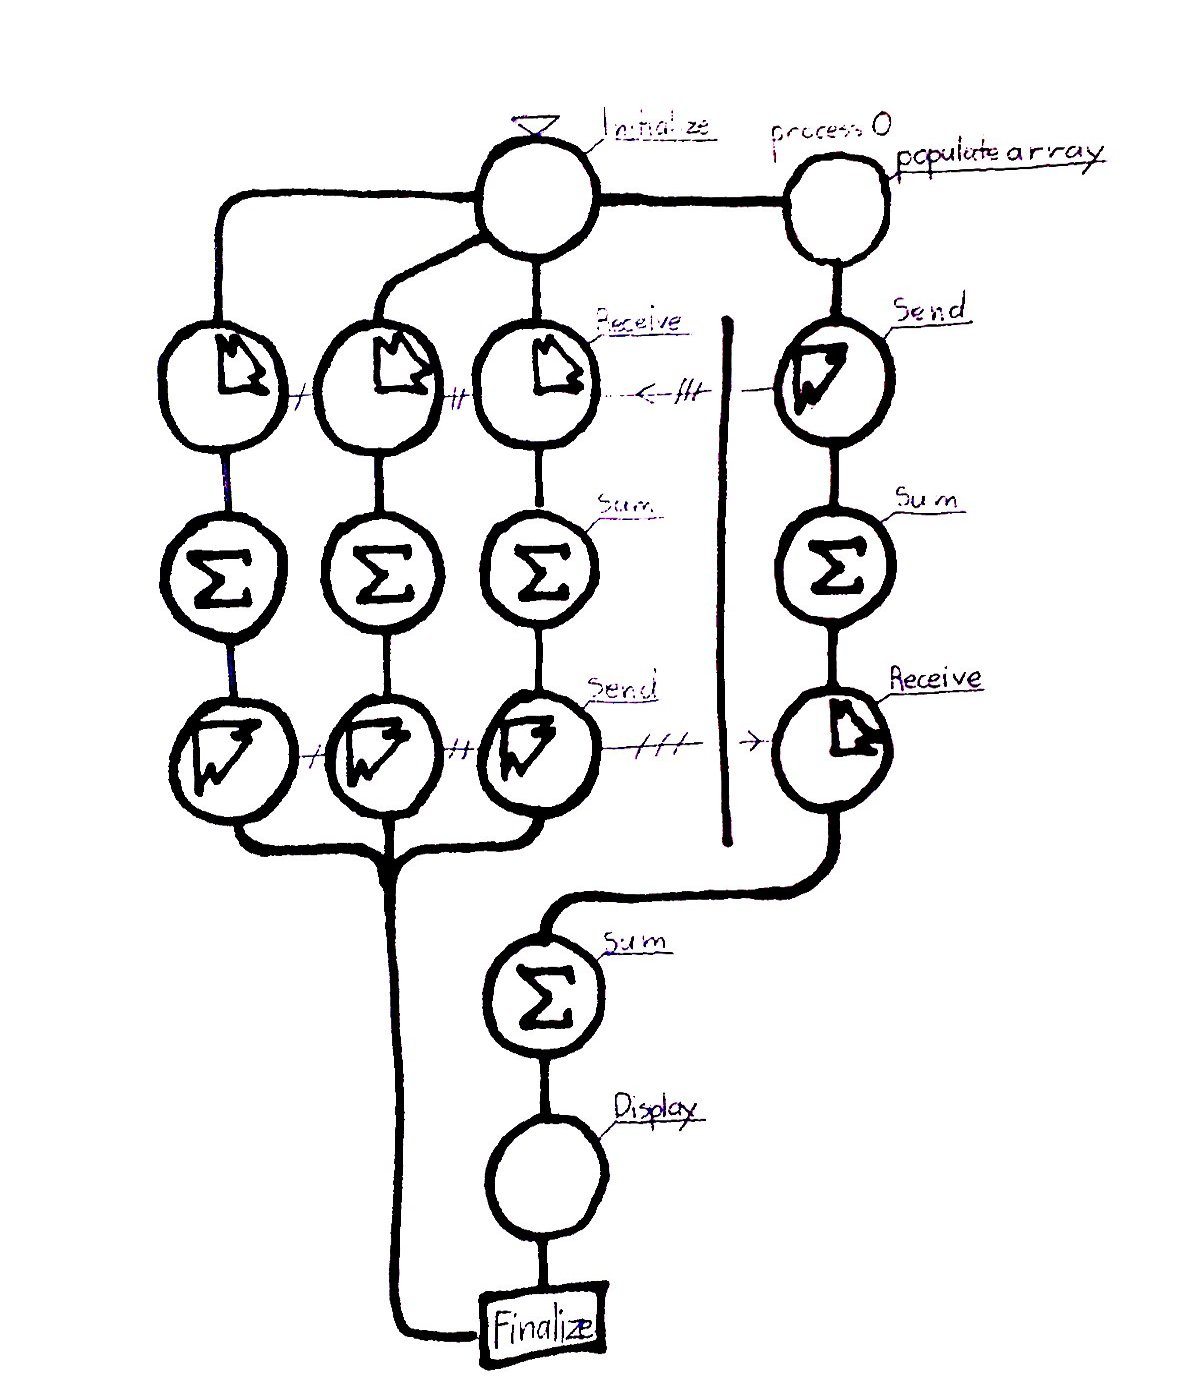
\includegraphics[width=\textwidth]{flytskjema1}
\caption{After each process is initiated and given rank, the primary process generates the full sequence alone. This is split into partitions, disjoint sets with full coverage, which is sent to each worker process. Each process, including the primary process will then take the sum of their sequence. Afterwards ay process not the primary one will proceed to send back the sum of its partition to the primary process which receives. The sums of the sums is then taken and displayed. }
\end{figure}


\lstinputlisting[language=C]{../oving4.c}
\lstinputlisting[language=C]{../mpisum.c}
%//\lstinputlisting[language=C]{../openmp_mpi.c}





\end{document}
